%%
%% Copyright 2007, 2008, 2009 Elsevier Ltd
%%
%% This file is part of the 'Elsarticle Bundle'.
%% ---------------------------------------------
%%
%% It may be distributed under the conditions of the LaTeX Project Public
%% License, either version 1.2 of this license or (at your option) any
%% later version.  The latest version of this license is in
%%    http://www.latex-project.org/lppl.txt
%% and version 1.2 or later is part of all distributions of LaTeX
%% version 1999/12/01 or later.
%%
%% The list of all files belonging to the 'Elsarticle Bundle' is
%% given in the file `manifest.txt'.
%%

%% Template article for Elsevier's document class `elsarticle'
%% with numbered style bibliographic references
%% SP 2008/03/01
%%
%%
%%
%% $Id: elsarticle-template-num.tex 4 2009-10-24 08:22:58Z rishi $
%%
%%
\documentclass[preprint,11pt,3p]{elsarticle}
\renewcommand{\baselinestretch}{1.5} 
%% Use the option review to obtain double line spacing
%% \documentclass[preprint,review,12pt]{elsarticle}

%% Use the options 1p,twocolumn; 3p; 3p,twocolumn; 5p; or 5p,twocolumn
%% for a journal layout:
%% \documentclass[final,1p,times]{elsarticle}
%% \documentclass[final,1p,times,twocolumn]{elsarticle}
%% \documentclass[final,3p,times]{elsarticle}
%% \documentclass[final,3p,times,twocolumn]{elsarticle}
%% \documentclass[final,5p,times]{elsarticle}
%% \documentclass[final,5p,times,twocolumn]{elsarticle}

%% if you use PostScript figures in your article
%% use the graphics package for simple commands
%% \usepackage{graphics}
%% or use the graphicx package for more complicated commands
%% \usepackage{graphicx}
%% or use the epsfig package if you prefer to use the old commands
%% \usepackage{epsfig}

\hyphenation{con-tainer con-tainers mari-time ge-neration consis-ting ite-ration ge-ne-ral}

\usepackage{enumitem}
\usepackage{amsmath}
\usepackage{graphics}
\usepackage{multirow}
\usepackage{floatrow}
\usepackage{subcaption}
\usepackage{pgfplots}

%% The amssymb package provides various useful mathematical symbols
\usepackage{amssymb}
%% The amsthm package provides extended theorem environments
%% \usepackage{amsthm}

%% The lineno packages adds line numbers. Start line numbering with
%% \begin{linenumbers}, end it with \end{linenumbers}. Or switch it on
%% for the whole article with \linenumbers after \end{frontmatter}.
%% \usepackage{lineno}

%% natbib.sty is loaded by default. However, natbib options can be
%% provided with \biboptions{...} command. Following options are
%% valid:

%%   round  -  round parentheses are used (default)
%%   square -  square brackets are used   [option]
%%   curly  -  curly braces are used      {option}
%%   angle  -  angle brackets are used    <option>
%%   semicolon  -  multiple citations separated by semi-colon
%%   colon  - same as semicolon, an earlier confusion
%%   comma  -  separated by comma
%%   numbers-  selects numerical citations
%%   super  -  numerical citations as superscripts
%%   sort   -  sorts multiple citations according to order in ref. list
%%   sort&compress   -  like sort, but also compresses numerical citations
%%   compress - compresses without sorting
%%
%% \biboptions{comma,round}

% \biboptions{}


\journal{European Journal of Operational Research}

%\numberwithin{equation}{section}
\allowdisplaybreaks

\begin{document}

\begin{frontmatter}

\title{Matheuristics for Slot Planning of Container Vessel Bays}


\author[itu]{Aleksandra Korach}
\ead{akor@itu.dk}

\author[op]{Berit Dangaard Brouer}
\ead{berit.dangaard.brouer@optivation.dk}

\author[itu]{Rune M{\o}ller Jensen\corref{cor1}}
\ead{rmj@itu.dk}

\address[itu]{IT University of Copenhagen, Rued Langgaards Vej 7, 2300 Copenhagen S, Denmark}

\address[op]{Optivation, Njalsgade 76, 2300 Copenhagen S, Denmark}


\cortext[cor1]{Corresponding author}

\begin{abstract}
Stowage planning is an NP-hard combinatorial problem concerned with loading a container vessel in a given port, such that a number of constraints regarding the physical layout of the vessel and its seaworthiness are satisfied, and a number of objectives with regards to the quality of the placement are optimized. The problem can be decomposed into phases, the latter of which, known as slot planning, involves loading the containers into slots of a bay. This article presents an efficient matheuristic for the slot planning problem. Matheuristics are algorithms using mathematical programming techniques within a heuristic framework. The method finds solutions for 96\% of 236 instances based on real stowage plans, 90\% of them optimally, with an average optimality gap of 4.34\% given a limit of one second per instance. This is an improvement over the results provided by previous work.
\end{abstract}

\begin{keyword}
%% keywords here, in the form: keyword \sep keyword
OR in Maritime Industry \sep Stowage Planning \sep Slot Planning \sep Matheuristics \sep Large Neighbourhood Search 
%% MSC codes here, in the form: \MSC code \sep code
%% or \MSC[2008] code \sep code (2000 is the default)
\end{keyword}

\end{frontmatter}

%%
%% Start line numbering here if you want
%%
% \linenumbers

%% main text
\section{Introduction}
\label{sec:Introduction}
With 90\% of general cargo nowadays carried by container vessels, maritime transport remains the foundation of international trade. These vessels travel on specific trade routes calling at different ports, where containers are unloaded and loaded according to a stowage plan. 

By providing an assignment of containers loaded at a given port to specific slots within bays of a container ship, stowage plans aim to maximise capacity utilisation and minimise operational costs. One crucial factor in achieving these objectives is the minimisation of \textit{overstowage}, i.e. a situation where a container to be unloaded is blocked by containers destined for later ports. Since stacks can only be accessed from the top, such containers need to be removed before a container underneath it can be retrieved. It is furthermore required that a good stowage plan satisfies a number of high-level constraints, pertaining to seaworthiness, stability requirements and stress limits of the vessel, as well as low-level constraints, concerned with stacking rules and capacity limits for stacks. All of these characteristics make generation of feasible and cost-efficient stowage plans a challenging endeavour.

Typically, stowage plans are manually prepared by stowage planners with an aid of graphical tools in the process known as \textit{stowage planning}. However, for the past few decades, the liner shipping industry has been confronted with a surge in demand for containerised transport of goods. The demands are being met by providing a higher frequency of service on the shipping routes and through deployment of ever larger vessels, now capable of carrying up to 19000 TEUs (Twenty-foot Equivalent Units). Plans for such vessels are still generated within mere hours before they call at a port, and under these time constraints stowage planners must be able to evaluate different forecast scenarios. Consequently, stowage planning is gradually becoming too cumbersome for humans, drawing industrial interest in the automation of this process.

State-of-the-art algorithms employed to solve the stowage planning problem generally apply a 2-phase approach, emulating the steps followed by stowage planners, as illustrated in Figure \ref{fig:decomposition}. Initially, a \textit{master planning} phase determines the distribution of containers into bay sections known as locations, while satisfying the high-level constraints. It is followed by a \textit{slot planning} phase, which is concerned with the assignment of containers in a given location to specific slots, in accordance with low-level stacking rules and limits. Based on the container load-list, vessel and port data, master planning produces a master plan for each location, which can subsequently be used as input to the slot planing module to generate the complete, final stowage plan.

\begin{figure}[ht]
\centering
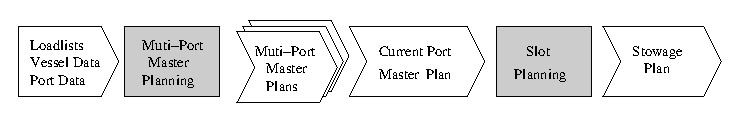
\includegraphics[width=1.0\linewidth]{Figures/quad.eps}
\caption{Decomposition of stowage planning into master planning and slot planning phases.}
\label{fig:decomposition}
\end{figure}


In this article, we build upon the approach presented in \cite{PDJB11, PDJB12, DJJRA12}, focusing on the slot planning stage. Although there exist fast, optimal methods for the slot planning problem \cite{DJJRA12}, in the context of stowing the whole vessel with potentially as many as 100 locations this task needs to be performed as fast as possible, opening the path for even faster, albeit heuristic solutions. We contribute to this cause in this article by presenting an efficient ruin-and-recreate matheuristic using an IP model (as presented in \cite{DPhD}) and based on a heuristic search framework. It builds upon an idea proposed by Prescott-Gagnon et al. \cite{PGDR-Math}, where a mathematical model is iteratively solved through branch-and-price in the re-creation phase of large neighbourhood search (LNS). To the best of our knowledge, no attempts at applying such a matheuristic to the problem at hand have been made to date. A battery of neighbourhoods were designed for the purpose of ruining a solution, initially obtained by a constructive heuristic, and then iteratively rebuilding it with a commercial IP solver. We apply the algorithm to solve the Container Stowage Problem for Below Deck Locations (\textit{CSPBDL}) introduced in \cite{DJJRA12}, and formulated by the authors in collaboration with a large liner shipping company. It is a representative, although slightly simplified, abstraction of the slot planning problem for bay locations found under deck. To provide a sound evaluation and a ground for comparison of methods, we have used the same set of instances as our predecessors \cite{DJJRA12}, adapted from genuine industrial stowage plans. It is evident from the results, that given a set of instances and a limited time frame, the matheuristic yields more solutions, and of higher quality, than the IP formulation alone when solved by a general-use solver, in a significantly decreased time. For a limit of 1~second, applying the matheuristic results in an average optimality gap of 4.34\% with instances solved within 106.16 seconds in total, as compared to a gap of 29.14\% achieved by the general-use solver within 140.77 seconds.

The remainder of this article is organised as follows. Section \ref{sec:Background} introduces background information and provides a detailed definition of the problem. It is followed by a literature review in Section \ref{sec:Literature}. Section \ref{sec:Model} presents the IP model used by the matheuristic during the re-creation procedure, while Section \ref{sec:ConstHeuristic} describes the placement heuristic employed to generate initial solutions. The matheuristic framework is examined in Section \ref{sec:Matheuristic}, and Section \ref{sec:Neighbourhoods} explores the designed ruin neighbourhoods. The details of experiments and their results can be found in Section \ref{sec:Experiments}, whereas Section \ref{sec:Conclusion} discusses conclusions and potential for further development.

\section{Background and Problem Statement}
\label{sec:Background}
A shipping container is a standardised piece of equipment universally used in international trade for transportation of non-bulk commodities, be it by land (trains, trucks) or water (container ships). Made of steel, they mostly come in three standard lengths of 20', 40', or 45' with a width of 8', although longer containers are also in use. Containers can be either 8'6" (\textit{standard-cube}, DC) or 9'6" high (\textit{high-cube}, HC), HC 20' containers are, however, rare. At a maximum, 20' and 40' containers can have a weight of about 24 and 30 tons. Due to the absence of inner supports, it is not allowed to stack 20' containers on top of 40' and 45' containers. Some cargo requires special considerations. \textit{Reefer} containers are intended for goods in need of refrigeration and must be placed near power plugs. \textit{DG} containers hold dangerous items and are bound by strict separation rules. \textit{Out-of-gauge} (OOG) containers are meant for goods exceeding their standard dimensions, and are usually stored in dedicated sections of the ship.

\begin{figure}[ht]
\centering
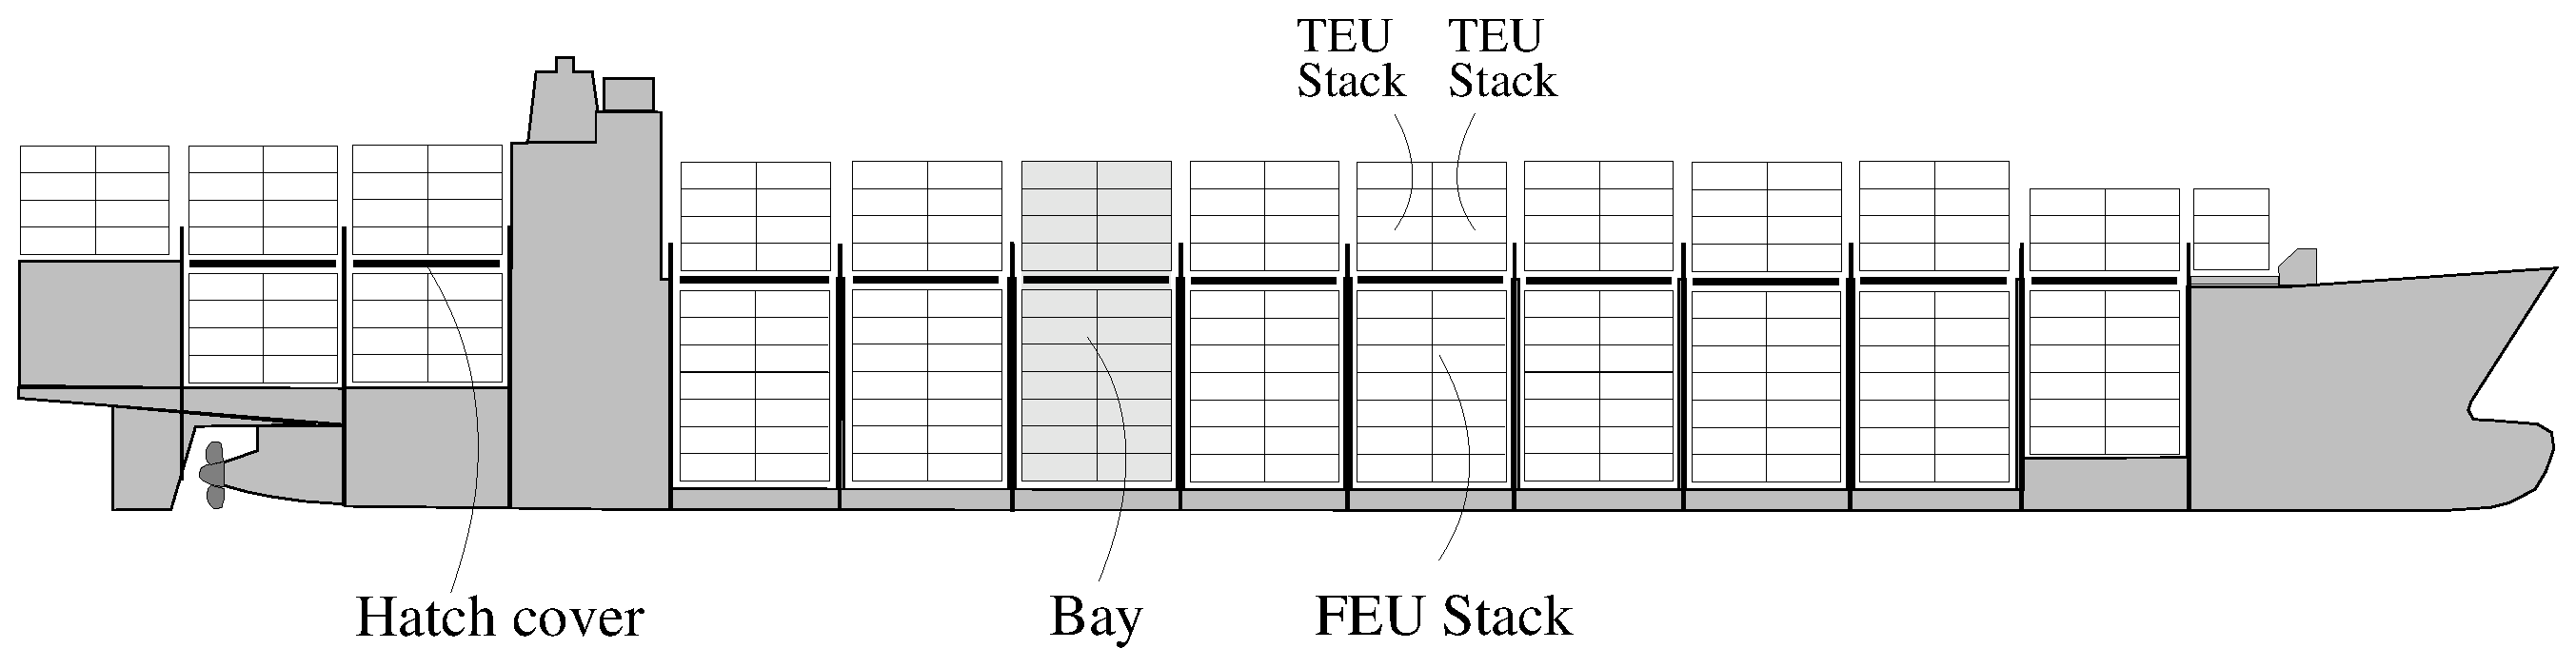
\includegraphics[width=1.0\linewidth]{Figures/vessel.eps}
\caption{Container vessel architecture.}
\label{fig:vessel}
\end{figure}

Container vessels are ships tailor-made for transporting containers, and their nominal capacity is given in Twenty-foot Equivalent Units (TEUs). As shown in Figure \ref{fig:vessel}, they are divided into sections called \textit{bays}, which consist of \textit{on-deck} and \textit{below-deck} parts separated by a \textit{hatch cover} -- a flat, waterproof barrier. Within bays, containers are organised into numbered \textit{stacks} bound by height and weight limits and comprised of \textit{cells} indexed by \textit{tiers}. Each cell may contain either a single 40', 45' container, or two 20' containers, an equivalent of 2 TEUs, with the exception of \textit{odd cells} with available space of 1 TEU. 45' containers are usually kept on deck. Cells are composed of 2 \textit{slots}, \textit{fore} and \textit{aft}, with the former situated towards the bow, and the latter to the stern of the ship. Some slots are fitted with power plugs to allow for stowage of reefers. Below deck, the safety of containers is guaranteed by \textit{cell guides}, while \textit{lashing rods} and \textit{twist locks} keep them in place on deck.

\begin{figure}[ht]
    \centering
    \begin{subfigure}[b]{0.35\textwidth}
        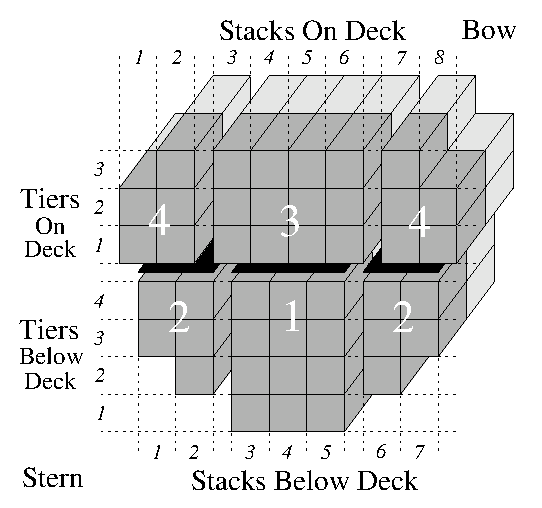
\includegraphics[width=\textwidth]{Figures/bay.eps}
        \caption{}
        \label{fig:bay}
    \end{subfigure}
    ~
    \begin{subfigure}[b]{0.28\textwidth}
        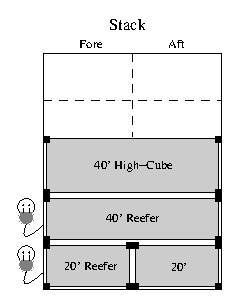
\includegraphics[width=\textwidth]{Figures/stack.eps}
        \caption{}
        \label{fig:stack}
    \end{subfigure}
    \caption{(a) A front view of a bay. (b) A side view of a container stack with power plugs.}\label{fig:bay_stack}
\end{figure}

In ports, quay cranes retrieve containers from and load them into bays. Containers are assigned to specific ports they are destined for, referred to as their \textit{port of discharge} (POD). Containers that remain on board, waiting to be unstowed in further ports, are known as \textit{remain-on-board} (ROB) containers, and need to be accounted for when preparing a stowage plan. Should a container bound for a later port be found above a container to be unloaded, the former is said to be \textit{overstowing} the latter. The necessity to unload and restow such containers prolongs the costly crane operation time and should be avoided, thus making overstowage minimisation one of the most important stowage planning objectives.

This article explores the problem of \textit{slot planning}, concerned with the assignment of containers in a bay location to specific slots on a vessel, where some cells may already be occupied by ROB containers. To this end, we utilise the abstraction presented in \cite{DJJRA12}, which was devised in collaboration with a liner shipping company -- the \textit{Container Stowage Problem for Below-Deck Locations} (\textit{CSPBDL}). The problem is argued to be NP-hard \cite{DJJRA12}. As justified by the authors, it is representative of the constraints and objectives present in the real-life problem. Due to high similarity of the problem elements between on-deck and below-deck locations, the presented approach could also be applied to the former likely with similar results \cite{DJJRA12}. The \textit{CSPBDL} formulation includes constraints pertaining to weight and height limits for stacks as well as stacking rules for 20' and 40' containers. Among the types of containers taken into consideration there are 20' and 40' containers of both DC and HC height. They can also be reefer or non-reefer. ROB containers may be present. A feasible \textit{CSPBDL} solution must be subject to the following rules \cite{DJJRA12}:

\begin{enumerate}[label=(\roman*), noitemsep]
    \item \label{constr:a} Assigned cells must form stacks (containers stand on top of each other in the stacks; they must have support from below).
    \item \label{constr:b} 20' containers cannot be stacked on top of 40' containers.
    \item \label{constr:c} A 20' reefer container must be placed in a reefer slot. A 40' reefer container must be placed in a cell with at least one reefer slot.
    \item \label{constr:d} The length constraint of a cell must be satisfied (some cells only hold 40' or 20' containers).
    \item \label{constr:e} The sum of heights and weights of the containers stowed in a stack are within the stack limits.
    \item \label{constr:f} All ROB containers must be stowed in their original slots and they cannot be swapped to any other slots.
    \item \label{constr:g} A cell must be either empty or with both slots occupied.
\end{enumerate}

Moreover, an optimal \textit{CSPBDL} slot plan must minimise the sum of the following objectives \cite{DJJRA12}:

\begin{enumerate}[label=(\alph*), noitemsep]
    \item \label{obj:a} Minimise overstows. A penalty of 1000 units is paid for each container overstowing containers below.
    \item \label{obj:b} Avoid stacks where containers have many different PODs. A penalty of 200 units is paid for each POD included in a stack.
    \item \label{obj:c} Keep stacks empty if possible. A penalty of 100 units is paid for each used stack.
    \item \label{obj:d} Avoid loading non-reefer containers into reefer slots. A penalty of 50 units is paid for each non-reefer container stowed in a reefer slot.
\end{enumerate}

Overstowage minimisation is of the greatest importance and hence incurs the highest cost. The objectives \ref{obj:b} through \ref{obj:d} are based on rules of thumb employed by stowage planners. Keeping containers clustered according to their POD and using as few stacks as possible helps increase capacity utilisation and decrease opportunities for overstowage in future ports. Minimising the number of non-reefers stowed in reefer slots allows for loading more reefer containers in later ports \cite{DJJRA12}. As reported in \cite{DJJRA12}, the penalty costs were consulted with the liner shipping partner. They are applied in the cost function.

\section{Literature Review}
\label{sec:Literature}
Slot planning can be either viewed as a phase or otherwise analysed as an integral part of the stowage planning problem. For this reason, a survey of approaches to the whole problem is crucial in understanding this last stage. 

Stowage planning can be either studied as a whole or decomposed into a hierarchy of sub-problems, which affords a division of methods into single-phase and multi-phase. To date, a variety of optimisation techniques have been applied to diverse formulations of the problem, e.g. mathematical programming (with use of linear or integer models), a selection of metaheuristics, as well as carefully tailored heuristics based on rules of thumb or observing human planners at work. The works often use differing models, making different assumptions about constraints and objectives, taking varying aspects of the problem into account, and presenting better or worse model accuracy. There is also a number of publications discussing theoretical issues of the stowage planning problem, e.g. its complexity (Tierney et~al. \cite{TPJ14}).

Multi-phase approaches tackle the problem of stowage planning through a hierarchical decomposition into phases which are then solved independently, and output of an earlier stage is treated as input to the subsequent stage. Literature shows that stowage planning is often divided into master and slot planning phases \cite{DPhD, PDJB11}, though other divisions have also been researched \cite{N13}. Many decomposition approaches stem from works by Wilson and Roach \cite{WR00}. Zhang et al. \cite{ZLJ05} present a 2-phase approach with a~Bin-Packing heuristic in the first one, and tabu search in the second. Min et al \cite{MLJYFA10A} describes a stowage planning system consisting of three modules: a stowage plan generator, a stability module, and an optimisation engine. In their study, Ambrosino et al. \cite{AAPS09, AAPS10, APS15} present variations on a 3-phase approach, combining a tailored heuristic for the first stage, an IP model or a constructive heuristic for the second, and either an iterative swapping heuristic or tabu search for the third phase. The work of Pacino et al. \cite{PDJB11} puts forward IP models for master planning, with slot planning solved by local search approaches. Li \cite{L12} attempted a 2-phase approach utilising an IP model and tabu search. Other contributions include work by Ning et al. \cite{N13} who distinguish 5 phases in their formulation; Lee et al. \cite{LFH15} introduce a 2-phase heuristic with objectives changing between phases.

Single-phase methods tackle the problem as a whole. Below follows a survey of such approaches and also those studies that focus only on a part of the problem.

There are relatively few studies where a constraint programming (CP) model was used for solving the stowage planning problem. Ambrosino and Sciomachen \cite{AS98} were the first to try -- they developed a CP model for the whole Master Bay Plan Problem (stowage planning). Later, Delgado et al. \cite{DJJRA12} presented a CP model for slot planning of below-deck locations.

A considerable amount of work utilises mathematical programming for solving the problem, including the study of Li et al. \cite{LTCD08} where a binary IP model for container stowage was presented and solved with a COIN-OR branch-and-bound algorithm. Pacino et al. \cite{PDJB12} developed an IP model for solving the master planning phase of the 2-phase approach, notably taking the modelling of ballast tanks into consideration. It was solved by a standard solver, as was the model for the slot planning phase introduced by Delgado et al. \cite{DJJRA12}. 

Matheuristics are optimisation methods integrating mathematical programming (MP) techniques into a heuristic framework. To date they have been successfully applied to a variety of problems, including vehicle routing problems, as presented in the survey by Archetti and Speranza \cite{AS14}. The survey also identifies various matheuristic paradigms. \textit{Decomposition approaches}, may divide the problem into parts, some of which may be solved with MP methods, or use MP to optimise a subset of objectives. \textit{Improvement heuristics} include \textit{one-shot methods}, where MP models are used to improve solutions found by other heuristsics, as well as \textit{approaches with MILP models for local optimisation}. The latter type embeds MP techniques as operators within a search algorithm, which can be used to explore the neighbourhood, as intensification tools, or as operators to complete a partial solution. Finally, some matheuristic approaches use \textit{branch-and-price/column generation} procedures to solve MILP models. The MIP model by Ambrosino et al. \cite{APS15} is iteratively solved with a 2-step relax-and-fix heuristic, making it the only matheuristic in this survey.

Many studies employ metaheuristics such as genetic algorithms or tabu search to tackle the problem, often in tandem with other heuristic approaches. Examples include an ant colony algorithm by Hern\'{a}ndez et al. \cite{H13}, a genetic algorithm by Zhang and Lee \cite{ZL15} or pareto clustering search by Ara\'{u}jo et al. \cite{AACS16}.

Apart from metaheuristics, tailor-made heuristics are often applied. In their study, Parre\~{n}o et al. \cite{PPAV16} developed a GRASP algorithm, the best-performing method for the \textit{CSPBDL} to date. We use the constructive heuristic proposed in their paper. The work of Ding and Chou \cite{DC15} constitutes another example.

Finally, some studies attempt to solve the stowage planning problem based on its connection to the 3D Bin Packing Problem, most notably Sciomachen and Tanfani \cite{ST03}, where the relationship between the two is discussed.

Since the approach taken in this article considers only the slot planning phase, its place is among the single-phase solutions in the above classification. The use of matheuristics situates it among both the IP and heuristic approaches.

\begin{table} [ht]
\begin{tabular}{rl}
    & \textbf{\textit{Sets}}\\
    $Q$& Containers to stow.\\
    $Q^{\{20, 40\}}$& 20' and 40' containers in $Q$.\\
    $M$& ROB containers.\\
    $J$& Stacks.\\
    $K_j$& Cells in stack $j$.\\
    $P$& Discharge ports.
\end{tabular}
\caption{Sets used in the IP model.}
\label{tab:IPSets}
\end{table}

\section{Integer Programming Model}
\label{sec:Model}

Below we present the IP model for the \textit{CSPBDL} problem, as introduced in \cite{DJJRA12, DPhD}. Although the considered objectives and constraints are the same as those presented in these studies, the use of the model is different. It is used by the matheuristic to solve unfixed parts of a solution. Tables \ref{tab:IPSets}, \ref{tab:IPConstants} and \ref{tab:IPVars} contain the explanation of symbols for sets and constants, as well as variables used in the model. Stacks $j$ in a given location are numbered from 1 to $|J|$, and each stack consists of $|K_j|$ cells $k$, numbered from 1. Similarly, containers $i$ are also numbered from 1, and PODs $p$ are numbered from 1 to $|P|$, ordered from the earliest to the latest.



\begin{table}[!ht]
\begin{center}
\begin{tabular}{rl}
    & \textbf{\textit{Constants}}\\
    $H^{C}_{i}$& Height of container $i$ in metres.\\
    $H^{S}_{j}$& Height of stack $j$ in metres.\\
    $W^{C}_{i}$& Weight of container $i$ in tons.\\
    $W^{S}_{j}$& Weight capacity of stack $j$ in tons.\\
    $R_{jk}$& Number of reefer plugs in cell $k$ of stack $j$.\\
    $R^{C}_{i}$& Indicates whether container $i$ is reefer.\\
    $A_{ip}$& Indicates whether container $i$ is discharged at port $p$.\\
    & If so, the value is $1$; $0$ otherwise.\\
    $C^v$& Penalty for a container overstowing containers below.\\
    $C^p$& Penalty for each POD used in a stack.\\
    $C^u$& Penalty for the use of a stack.\\
    $C^r$& Penalty for stowing a non-reefer container in a reefer slot.
\end{tabular}
\end{center}
\caption{Constants used in the IP model.}
\label{tab:IPConstants}
\end{table}

\begin{table} [!ht]
\begin{center}
\begin{tabular}{rl}
    & \textbf{\textit{Variables}}\\
    $c_{jki} \in \{0, 1\}$& Container $i$ stowed in cell $k$, stack $j$.\\
    $o_{i} \in \{0, 1\}$& Container $i$ overstowing other containers.\\
    $d_{jp} \in \{0, 1\}$& At least one container in stack $j$ is discharged at port $p$.\\
    $e_{j} \in \{0, 1\}$& Stack $j$ is in use (i.e., stack $j$ is non-empty).\\
    $\delta_{jkp} \in \{0, 1\}$& Container below cell $k$, stack $j$ is discharged before port $p$.
\end{tabular}
\end{center}
\caption{Variables used in the IP model.}
\label{tab:IPVars}
\end{table}

Penalties in the constants table take the values specified in the problem objectives \ref{obj:a} through \ref{obj:d}. The $c$ variables are decision variables representing the slot plan, while the auxiliary variables are utilised for calculating the objective components. Based on these elements, the following IP model is defined:

\small
\begin{equation}
\label{eq:objective}
\begin{aligned}
\min \qquad  & C^v \sum_{i \in Q} o_i + C^p \sum_{j \in J} \sum_{p \in P-\{1\}} d_{jp} + C^u \sum_{j \in J} e_j \\ 
            & + C^r \sum_{j \in J}\sum_{k \in K_j}(R_{jk} \sum_{i \in Q^{40}} c_{jki}(1 - R^{C}_{i}) + \sum_{i \in Q^{20}} c_{jki}(\frac{1}{2}R_{jk} - R^{C}_{i})) 
\end{aligned}
\end{equation}
\begin{alignat}{15}    
    \text{s.t.} & & \nonumber \\
                & \frac{1}{2} \sum_{i \in Q^{20}} c_{j(k-1)i} + \sum_{i \in Q^{40}} c_{j(k-1)i} - \sum_{i \in Q^{40}} c_{jki} \geq 0 \enskip && \forall j \in J, \enskip k \in K_j - \{1\} \label{eq:constr1}\\
                & \sum_{i \in Q^{20}} c_{jki} - \sum_{i \in Q^{20}} c_{j(k-1)i} \leq  0 && \forall j \in J, \enskip k \in K_j - \{1\} \label{eq:constr2}\\
                & \frac{1}{2} \sum_{i \in Q^{20}} c_{jki} + \sum_{i \in Q^{40}} c_{jki} \leq  1 && \forall j \in J, \enskip k \in K_j \label{eq:constr3}\\
                & \sum_{j \in J} \sum_{k \in K_j} c_{jki} = 1 && \forall i \in Q \label{eq:constr4}\\
                & \sum_{i' \in Q^{20}} c_{jki'} - 2c_{jki} \geq  0 && \forall j \in J, \enskip  k \in K_j, \enskip i \in Q^{20} \label{eq:constr5}\\
                & \sum_{i \in Q} R^{C}_{i}c_{jki} - R_{jk} \leq  0 && \forall j \in J, \enskip k \in K_j \label{eq:constr6}\\
                & \sum_{k \in K_j} \sum_{i \in Q}  W^{C}_{i}c_{jki} \leq W^{S}_{j} && \forall j \in J \label{eq:constr7}\\
                & \sum_{k \in K_j} (\frac{1}{2} \sum_{i \in Q^{20}} H^{C}_{i}c_{jki} + \sum_{i \in Q^{40}} H^{C}_{i}c_{jki}) \leq H^{S}_{j} && \forall j \in J \label{eq:constr8}\\
                & \sum_{k'=1}^{k-1} \sum_{p'=2}^{p-1} \sum_{i \in Q} A_{ip'}c_{jk'i} - 2(k - 1)\delta_{jkp} \leq 0 && \forall j \in J, \enskip  k \in K_j - \{1\},  \label{eq:constr9}\\
                & && p \in P - \{1, 2\} \nonumber\\
                & A_{ip}c_{jki} +  \delta_{jkp} - o_i \leq  1 && \forall j \in J, \enskip k \in K_j \label{eq:constr10}\\
                & && p \in P, \enskip i \in Q \nonumber\\
                & e_j - c_{jki} \geq  0 && \forall j \in J, \enskip k \in K_j \enskip i \in Q \label{eq:constr11}\\
                & d_{jp} - A_{ip}c_{jki}  \geq  0 && \forall j \in J, \enskip k \in K_j \label{eq:constr12}\\ 
                & && p \in P, \enskip i \in Q \nonumber\\
                & c_{jki} = 1 && \forall (j,k,i) \in M \label{eq:constr13}
\end{alignat}
\normalsize

The objective function is defined as a weighted sum of the \textit{CSPBDL} problem objectives, with the $o_i$, $d_{jp}$ and $e_j$ variables summed and multiplied by their respective penalties. As for the reefer objective, the number of stowed non-reefer containers is calculated for each cell with reefer slots. Seeing as 40' containers require only a single reefer slot per cell, they need to be considered independent of 20' containers. 
Constraint \eqref{eq:constr1} guarantees that 40' containers do not hang in the air \ref{constr:a}, demanding either two 20' or one 40' container be present below a cell holding a 40' container, with the exception of the bottom cell. Similarly, inequality \eqref{eq:constr2} ensures that two 20' containers are always present beneath a cell with 20' containers \ref{constr:b}. The fact that no more than two 20' or one 40' container can be stowed in a cell is enforced by constraint \eqref{eq:constr3}, while inequality \eqref{eq:constr4} requires all containers to be stowed in exactly one cell. Since a cell must always be either fully occupied or empty \ref{constr:g}, constraint \eqref{eq:constr5} demands the number of 20' containers in a cell to be either 0 or 2. Reefer containers are forced to be stowed in slots with reefer plugs \ref{constr:c} by constraint \eqref{eq:constr6}. The weight and height stack limits \ref{constr:e} are constrained by inequalities \eqref{eq:constr7} and \eqref{eq:constr8} respectively. In constraint \eqref{eq:constr9}, the $\delta_{jkp}$ variables are defined, and then used in inequality \eqref{eq:constr10} to assign correct values to the overstowage variables $o_i$. Variables $e_j$ and $d_{jp}$ require lower bounds to be set for them, which is accomplished by constraints \eqref{eq:constr11} and \eqref{eq:constr12} in the order given. Finally, constraint \eqref{eq:constr13} assigns ROB containers to their original positions \ref{constr:f}.

Additionally, the model comprises linear cuts to remove non-integer values assigned to $\delta$ variables from consideration, which is attained through the use of a Linear Programming relaxation \cite{DJJRA12}:
\small
\begin{alignat}{4} 
    \quad & A_{ip'}c_{jk'i} \leq \delta_{jkp} && \forall j \in J, \enskip  k \in K_j, \enskip p \in P, \enskip i \in Q, \enskip k' \in K', \enskip p' \in P' \label{eq:constr14}\\
    \quad & \frac{1}{2} \sum_{i \in Q'^{20}_{p}} c_{jk'i} \leq \delta_{jkp} \enskip && \forall j \in J, \enskip k \in K_j, \enskip p \in P, \enskip k' \in K' \label{eq:constr15}\\
    \quad & \sum_{i \in Q'^{40}_{p}} c_{jk'i} \leq \delta_{jkp} && \forall j \in J, \enskip k \in K_j, \enskip p \in P, \enskip k' \in K' \label{eq:constr16}\\
    \quad & \sum_{k'=1}^{k-1} A_{ip'}c_{jk'i} \leq \delta_{jkp} \enskip && \forall j \in J, \enskip k \in K_j, \enskip i \in Q, \enskip p \in P, \enskip p' \in P' \label{eq:constr17}
\end{alignat}
\normalsize

where $K' = \{k'|k' \in \{1, \ldots, k-1\}\}$, $P' = \{p'|p' \in \{2, \ldots, p-1\}\}$, and $Q'^{20}_{p}$ with $Q'^{40}_{p}$ describing the sets of, accordingly, 20' and 40' containers with POD earlier than $p$. Constraint \eqref{eq:constr9} is decomposed into a semantically equivalent set of inequalities \eqref{eq:constr14}. It is then expanded in cuts \eqref{eq:constr15} through \eqref{eq:constr17}, by including considerations of containers unloaded before port $p$, separately for 20' \eqref{eq:constr15} and 40' \eqref{eq:constr16} containers, as well as all cells below cell $k$ \eqref{eq:constr17}. \cite{DJJRA12}

\section{Constructive Heuristic}
\label{sec:ConstHeuristic}
Recall that the presented matheuristic approach comprises an LNS algorithm, where in every iteration solutions are partially ruined and rebuilt using a general-use mathematical solver. The search algorithm requires an initial solution as input that needs to be generated fast. For this purpose we employ a constructive heuristic described by Parre\~{n}o et al. \cite{PPAV16}. Below we present the details of this algorithm.

The heuristic follows an iterative process consisting of three steps preceded by an initialisation step. It takes the following elements as input: a list of ROB containers $C_R$ for the given instance, a list $C$ of containers to stow and a list $S$ of stacks. Additionally, each stack $s \in S$ is associated with a list $K_s$ of cells it consists of. The output of the constructive heuristic is an initial stowage plan. In each iteration, the heuristic selects a stack from $S$, and considers its lowest empty cell. Next, a container is chosen from among the $C$ list, so that its assignment to the selected stack and cell is feasible. When there are no more containers to stow or the remaining containers cannot be feasibly stowed in the available cells, the process is terminated. Finally, the left-over containers are placed in the remaining empty cells.

During initialisation, ROB containers are placed into their positions, and the other aforementioned lists are sorted. Stacks in $S$ are ordered first according to whether they are empty, in which case they appear last. Then they are sorted by the number of cells available for loading, in non-increasing order with empty stacks appearing last. The rationale is to minimise the number of stacks in use. 
%% RMJ: But isn't the last sorting then putting empty stacks first?
As for containers, an ordering is imposed based on their port of discharge, length, whether they are reefers, and their height class. Containers with later PODs are considered first to avoid overstowage. With regards to length, 20' containers appear first as they cannot be stowed on 40' containers. Then, reefers are considered before others, and finally HC containers before DCs.   

In the first step of the iterative process, the heuristic chooses the appropriate stack and cell. Initially, the first stack from $S$ is selected. Then, if the stack is filled or there are currently no containers that can be stowed in it, the algorithm moves on to the next stack. The stacks are revisited in the same order, considering that, as containers are loaded, some limits preventing other containers from being stowed in a given stack may be lifted, now permitting their placement (see conditions \ref{con:height} and \ref{con:plugs} below). 

The second step manages the choice of containers for stowing in a selected cell. In order for a container to be legally stowed in the cell, it must satisfy a few conditions:
\begin{enumerate}[noitemsep]
    \item \textbf{Weight Limit}: The total weight of the stack including the weight of candidate containers cannot exceed its weight limit.
    \item \label{con:height} \textbf{Height Limit}: The total height of the stack including the height of candidate containers cannot exceed its height limit. Furthermore, special rules apply when the candidate is an HC container. If assigning the candidate to the given cell reduces the number of DC containers that could otherwise be stowed in this stack, it cannot be loaded. However, the condition is only applicable if there are more standard-height containers with the same POD as the HC container, as it is more important to limit the number of PODs in a stack than to optimally utilise stack volume.
    \item \textbf{Length Class}: Some cells only accept containers of certain length. Length of a container must agree with cell restrictions. Secondly, 20' containers cannot be stowed in the selected cell if there is a 40' container underneath it. Moreover, a 20' container can only be loaded into the cell if there is another 20' container in $C$ that can also be feasibly stowed in that cell.
    \item \label{con:plugs} \textbf{Power Plugs}: Depending on the number of reefer slots in the cell,
    \begin{description}[noitemsep]
        \item \textit{0 reefer slots}: the candidate must be either a 40' or a 20' non-reefer container; in the latter case a matching \textit{non-reefer} container must be found. 
        \item \textit{1 reefer slot}: the candidate must be either a 40' or a 20' reefer; in the latter case a matching \textit{non-reefer} container must be found.
        \item \textit{2 reefer slots}: the candidate must be either a 40' or a 20' reefer; in the latter case, a matching \textit{reefer} container must be found.
    \end{description}
    Nevertheless, if there are no more reefer containers in $C$, non-reefers can also be loaded.    
\end{enumerate}

In the last step, the algorithm updates the list states. The container(s) selected in the previous step are removed from $C$  and the values of stowed stack weights and heights are altered as required. 

As mentioned above, after the iterative process is terminated, the remaining containers are placed in the first empty cells found, regardless of other constraints, and marked as violations. In consequence, the resulting solution may be infeasible.

\section{Matheuristic}
\label{sec:Matheuristic}
While designing our approach, we took example from the study by Prescott-Gagnon et al. \cite{PGDR-Math}, to use an improvement matheuristic which utilises an IP model for search optimisation, with LNS \cite{PR-LNS} as the metaheuristic framework. The reason is that LNS search methods lend themselves very well to complex problems with structure akin to that of slot planning. LNS follows a two-step 'ruin-and-recreate' procedure, where parts of a solution $x$ are iteratively destroyed (unfixed, ruined) and then rebuilt, implicitly defining its neighbourhood, $N(x)$. Ruining and reconstruction is accomplished by two sets of destroy $\Omega^{-}$ methods (\textit{destructors, destroyers, ruiners}) and rebuild $\Omega^{+}$ methods. By substituting the reconstructive methods with the use of a general-purpose MIP solver, we turn the LNS into a matheuristic. Below we discuss the overall design of the algorithm.

\subsection{Pre-search Initialisation}
As a first step, the method creates an IP model of the given instance. It is a one-time procedure, and the same model is later reused within search. To provide a basis for improvements during search, the fast constructive heuristic presented in Section \ref{sec:ConstHeuristic} is used to generate an initial solution. The cost of that solution is then calculated according to the model's cost function $c(x)$, as required by the search algorithm for comparison. The obtained solution is subsequently presented as input to the search method. 

\subsection{Matheuristic Large Neighbourhood Search}
Given that the re-creation step could never produce a solution of worse quality than the destroyed one, the LNS framework can be viewed as a hill climber with complex neighbourhoods. The presented approach is an any-time method that is terminated after a time limit is reached. An iteration limit and a non-improving iteration limit further restrict the algorithm's runtime. In the course of each iteration, we first consider the feasibility of the input solution $x$. If the solution is infeasible, all containers that violate constraints are unstowed. Next, the method randomly selects a destructor from $\Omega^{-}$, which then commences to unload whole stacks (or their parts) based on its underlying selection principle. How much is destroyed depends on the size of the input instance. Nevertheless, it should be noted that if many violations were present, a considerable part of the solution may have to be rebuilt. Thus, the matheuristic is strongly reliant on the quality of the constructive method. By adding auxiliary constraints to the model, the remaining containers are set as fixed, and re-creation is performed using a MIP solver, producing a neighbouring solution $x'$. If the repaired solution is infeasible, the matheuristic will continue to unstow additional stacks to allow a feasible solution to be constructed. After reconstruction, the auxiliary constraints are removed, and the solution quality is evaluated. If $c(x') \leq c(x)$ the update $x = x'$ is performed, and $x'$ marked as the best solution $x^b$ if the cost of $x'$ is strictly lower. The process continues until a given time limit, an iteration limit or a non-improving iteration limit is reached. During the course of search the remaining time is constantly updated, so that the solver does not run overdue.

To restrict the degree of destruction, all destroyers are allowed to unfix a random number of stacks between a minimum of 2 and a maximum of 50\% of all eligible stacks (the number of stacks in the instances varies from 2 to 10). If the number of stacks is 3, two stacks are destroyed. A stack is eligible for destruction, if it contains non-ROB containers. Preliminary tests revealed that a maximum of 50\% is a good compromise for the trade-off between destruction size and search time. Setting the limit to 25\% resulted in a slight speed gain and a drop in performance, while setting it to 75\% caused longer running times without a clear gain in solution quality.

\section{Destructors}
\label{sec:Neighbourhoods}
Each ruin method tries to address specific issues within the current solution, attempting to minimise relevant elements of the objective function. For the purposes of the matheuristic, several destructors were designed and are presented in this section.

In an article about adaptive large neighbourhood search \cite{PR-ALNS}, Pisinger and Ropke distinguish a few destroyer types: random-removal, worst-removal and related-removal. When applied to our problem, \textit{Random-removal} methods select stacks at random. \textit{Worst-removal} ruiners choose stacks that are the worst according to some criterion, e.g. have the most killed space. Finally, \textit{related-removal} destructors define a relationship between stacks, and unfix the ones that are related. We have designed and tested 2 random-removal, 3 worst-removal and 4 related-removal methods.

\subsection{Destructors related to the 'keep stacks empty' objective, \ref{obj:c}}
Starting with the most general objective, these ruin methods aim at maximising volume utilisation within stacks to accommodate as many containers as possible or necessary. The first three are general-use, applicable to all instances.

\textbf{Worst-removal: Most killed space.} As the name indicates, this algorithm chooses to destroy the stacks where volume (height) is poorly utilised - the most space is killed. The stacks are sorted in descending order according to the difference between their maximum height and their current height. Thus, partially filled stacks are selected first, potentially allowing them to be consolidated.

\textbf{Related-removal: Volume vs. weight.} The following heuristic juxtaposes heavy stacks with space for more containers but limited by weight, with the ones that are already volume-efficient, but could accept heavier containers instead. This is accomplished by sorting. Afterwards, stacks are selected by alternating between both head and tail of the list.

Stacks are sorted with respect to their \textit{current volume/weight ratio}, which is calculated by dividing the current weight of a stack by its current height. The \textit{perfect ratio} is defined by dividing the maximum weight by the maximum height, and describes the ratio that a stack would have if it was both volume- and weight-efficient. The algorithm orders the stacks according to the difference between these two ratios, ascending. A positive value indicates that so far a stack has accepted more weight for its current volume than the perfect ratio would suggest, while a negative value signifies the opposite. Therefore, at the head of the sorted list of stacks we would have stacks skewed to the heavier side, and at the tail - to the lighter.

Seeing as the ratio calculation is irrespective of the number of containers loaded, it is evident that partially filled stacks can also be chosen, and thus possibly consolidated.

\textbf{Related-removal: Volume vs. weight, version 2.} The only difference between this ruin method and the previous one is the sorting principle. Stacks are sorted first by height in a descending order, then by weight in an ascending order. As this sorting includes stacks with low volume (height) utilisation, it also allows partially filled stacks to be selected.

\textbf{Related-removal: HC/DC}. This destructor investigates the distribution of HC vs. DC containers within a solution, and is applicable if both HC and DC containers are present in the cargo mix. Its behaviour varies based on which type is dominant. As with the previous destroyer, the algorithm sorts the stacks depending on some criterion, and then selects stacks from both ends. 

Before proceeding, it is necessary to introduce a few concepts. \textbf{Free HC capacity} is the number of containers a stack can accept without the necessity to \textit{kill} any DCs, i.e. waste space that could have been taken by an additional DC container. \textbf{Extra HC capacity} are additional HC containers that can be stowed after killing one extra DC space. \textbf{Current HC capacity} is the number of HC containers that can still be loaded without killing any \textit{more} DC containers. A \textbf{perfect HC/DC cargo mix} describes a situation, where the cargo contains a number of HC containers equal to the sum of free HC capacities of all stacks within a location and the rest of containers are DC (see Figure \ref{fig:hcdc}). This allows for a maximum volume utilisation. 

\begin{figure}[ht]
\floatbox[{\capbeside\thisfloatsetup{capbesideposition={right,top},capbesidewidth=0.6\linewidth}}]{figure}[\FBwidth]
{\caption[Illustration of perfect and imperfect HC/DC mix in stacks.]{Illustration of perfect and imperfect HC/DC mix in stacks. Stack \textit{(a)} holds 2 DCs and 1 HC container, a total 26'6'' of height. It fully utilises its free HC capacity, and no space is wasted. Stack \textit{(b)} does not, and thus some space is left unused. 2 HCs in stack \textit{(c)} exceed its free HC capacity, causing one DC space to be killed. It follows, that an ideal HC/DC mix for these stacks is 3, although one HC from stack \textit{(c)} should be swapped with a DC in \textit{(b)}, allowing for an additional DC container to be stowed in \textit{(c)}.}\label{fig:hcdc}}
{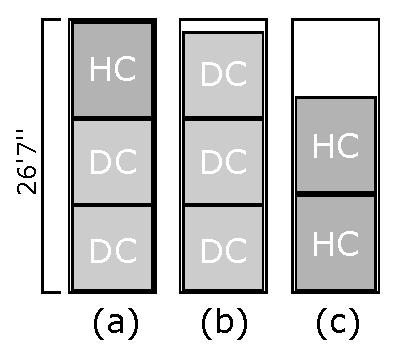
\includegraphics[width=0.7\linewidth]{Figures/hcdc_stacks.eps}}
\end{figure}

We consider three situations:
\begin{enumerate}[noitemsep]
    \item The cargo contains an ideal mix of HCs and DCs, i.e. the stacks can accept all of the HCs without the necessity to kill any DCs - their free HC capacity is enough.
    \item The cargo has fewer HC containers than the stacks could accept without killing any DCs; as a result, some stacks won't need to stow any HCs - their free HC capacity is more than enough.
    \item The cargo has more HCs than can be stowed without killing DCs; some have to be killed to accommodate for extra HCs - the free HC capacity of stacks is not enough.
\end{enumerate}

For the perfect mix, the aim is to ensure the stacks contain exactly the number of HCs they can fit so that no space is killed. The idea in the second case is to put the HCs in as few stacks as possible. These two situations can be dealt with together, since the goal of both is essentially the same: ensuring full utilisation of the free HC capacity in stacks by moving containers from stacks exceeding this capacity or not utilising it fully. It can be accomplished by imposing the same ordering on the stacks. For each stack, we calculate the difference between their capacity to stow HCs freely and the number of currently stowed HCs. We use the result as a sorting principle. 

Last but not least, if there are more HCs in the mix than the perfect number, a sound intention is to minimise the number of stacks with killed DC space, trying to fully utilise their HC capacity. Stacks where no DC space is killed and that cannot accept more HCs without killing DCs are placed in a separate list. The algorithm sorts the remaining stacks according to 3 criteria. First, it checks whether there are any stacks with fully utilised HC capacity and DC kills. If so, they are pushed to the end. Next, the heuristic sorts the stacks by the quantity of killed DCs (ascending), and by their current HC capacity (ascending). This way stacks with almost perfectly utilised HC capacity are juxtaposed with stacks that have most killed DC containers and poorly utilised HC capacity. Removing an HC container from the latter can potentially result in restoring DC space. 

We only select stacks from the auxiliary list if the algorithm chooses to destroy more stacks than available in the primary list. The order in the list is random.

\subsection{Destructors related to the 'overstowage' \ref{obj:a} and 'multiple POD' \ref{obj:b} objectives}
These destructors apply only to instances with more than one POD.

\textbf{Worst-removal: Number of overstowing containers.} The destructor unstows stacks with the highest quantity of containers that overstow others. It may be useful for situations when there is more than a single stack with overstowing containers. The order of stacks with the same number of overstowing containers is randomised.

\textbf{Worst-removal: Stacks with multiple PODs.} The algorithm unfixes the stacks with most varied PODs, as it might be possible to purify some stacks or at least reduce the number of different PODs they contain. In case of many stacks with the same number of PODs, we resolve the conflict by considering the stacks with the most significantly dominant POD first. The rationale is, that if there is a dominant POD in a stack, the algorithm may destroy it along with another one where a different POD is dominant, potentially allowing both, or one of them, to be purified by getting rid of the less numerous PODs.

\subsection{Destructor related to the 'reefer' objective, \ref{obj:d}}
\textbf{Related-removal:} This destroyer is only relevant in situations where there are more reefer slots than reefer containers.

In some cases, we might want to fully utilise reefer plugs of a stack instead of having reefers distributed unevenly between stacks. This could allow non-reefer containers to be stowed above the tiers with reefer plugs, imposing no penalty, moving them from other stacks and potentially saving a stack. The destruction is performed so that stacks with most, but not all, reefer slots taken are juxtaposed with those, where reefer plugs are so far poorly utilised. This is done by sorting the stacks according to a ratio of plugs taken to all plugs in a stack. Stacks with no reefer slots or all reefer slots in use are pushed to an auxiliary list.

Just like with the HC vs. DC destroyer, if the algorithm chooses to destroy more stacks than present in the main list, the remaining stacks are chosen from the separate list. The ordering of these stacks is random. 

\subsection{Random destroyers}
\textbf{Full-Stack Random.} The destroyer randomly chooses a set of eligible stacks to unfix.

\textbf{Two stacks with partial destruction.} This destructor ruins only two stacks at a time. If the number of stacks eligible for unstowing equals 2, random halves (upper or lower) of both stacks are unfixed.

\section{Experiments}
\label{sec:Experiments}
All experiments were performed on a Windows 10 machine with a 2-core 2.0 GHz Intel Core i7-4510U processor and 8.0 GB RAM. The matheuristic was implemented in C++, with the IP model implemented in Gurobi 6.5.1. It was evaluated on a set of 236 instances, each representing a location with a load list and derived from real stowage plans. These are the same instances as the ones used in \cite{DJJRA12}.

To facilitate a comparison with the results of previous studies, the instances were grouped into classes according to their features, as presented in \cite{DJJRA12} and \cite{PPAV16}. Table \ref{tab:instances} summarises the groups, giving details about the number of instances, the TEU-capacity of locations, the number of containers to stow, and the presence of certain features - 20', 40', reefer and high-cube containers, as well as the number of instances with either 1, 2, or 3 and more PODs.

\begin{table}[ht]
\scriptsize
\centering
\resizebox{\columnwidth}{!}{
\renewcommand{\arraystretch}{0.8}
\begin{tabular}{c c c c c c c c c c c c c c c}
    \hline
    \multirow{2}{*}{Class} & \multirow{2}{*}{\#} & \multicolumn{3}{c}{Cap. (TEUs)}  & \multicolumn{3}{c}{\#Cont. (TEUs)} & \multirow{2}{*}{40's} & \multirow{2}{*}{20's} & \multirow{2}{*}{R} & \multirow{2}{*}{HC} & \multicolumn{3}{c}{\#POD}  \\
    & & min & avg & max & min & avg & max & & & & & 1 & 2 & $\geq$ 3 \\
    \hline \hline
    1 & 13 & 16 & 63 & 116 & 8 & 54 & 116 & $\times$ & & & & 13 & & \\
    2 & 22 & 8 & 68 & 168 & 8 & 52 & 136 & & $\times$ & & & 22 & & \\
    3 & 13 & 30 & 74 & 124 & 8 & 68 & 124 & $\times$ & $\times$ & & & 13 & &\\
    4 & 78 & 6 & 79 & 208 & 2 & 63 & 202 & $\times$ & & & $\times$ & 78 & &\\
    5 & 36 & 38 & 97 & 176 & 8 & 81 & 170 & $\times$ & $\times$ & & $\times$ & 36 & &\\
    6 & 15 & 42 & 73 & 172 & 16 & 46 & 74 & $\times$ & & $\times$ & & 15 &\\
    7 & 14 & 72 & 147 & 204 & 24 & 117 & 202 & $\times$ & $\times$ & $\times$ & $\times$ & 14 & &\\
    8 & 14 & 40 & 96 & 148 & 40 & 87 & 136 & $\times$ & & $\times$ & $\times$ & & 14 & \\
    9 & 17 & 44 & 124 & 220 & 36 & 111 & 200 & $\times$ & $\times$ & $\times$ & $\times$ & & 15 & 2\\
    10 & 8 & 72 & 122 & 176 & 10 & 93 & 156 & $\times$ & & $\times$ & $\times$ & & 6 & 2\\
    11 & 6 & 48 & 101 & 176 & 28 & 84 & 148 & $\times$ & $\times$ & $\times$ & $\times$ & & 3 & 3\\
    \hline
\end{tabular}
}
\caption{Instance classes.}
\label{tab:instances}
\end{table}

A series of tests with increasing time limits was performed on the algorithm, measuring time performance, the average gap, the percentage of solutions found, and the number of instances solved to optimality. Time limit was gradually increased from 1 to 10 seconds, with 1-second steps. A maximum of 15 iterations and 5 non-improving iterations were chosen as additional stopping criteria.

\subsection{Comparison of different ruin methods}
We first examine the performance of different destructors and their mixes presented in Section \ref{sec:Neighbourhoods}, considering the general and feature-specific methods separately.

To begin with, let us focus on the general destroyers, which include the Random and Two-Stack Random (\textit{2-Random}) methods as well as the three general-use destructors related to objective \ref{obj:c}: Most Killed Space (\textit{MKS}) and the ratio and non-ratio version of Volume vs. Weight (\textit{VW} and \textit{VWR}) methods. In addition, two mixed sets were tested, containing 3 destructors each. The first mix pool included the VWR, MKS and Random ruiners (VWR Mix), while the other one contained VW instead of VWR (VW Mix). The results show, that neither of them is clearly better than the other. Table \ref{tab:general} presents the results for all of the variants, while Figure \ref{graph:generals} shows a performance graph of the best random, the best non-random destroyer and the VW mix of destroyers for the range of 1 - 10s time limits. 

\begin{figure}
\centering
\begin{subfigure}{.45\linewidth}\centering
\begin{tikzpicture}
\pgfplotstableread{Data/Generals-Gap.dat}{\ipchmath}
\begin{axis}[
                width=\linewidth,
                scale only axis, 
                minor tick num=3,
                xtick={0,1,...,10}, 
                ytick={0,1,2,3,4,5,6},
                tick label style={font=\scriptsize},
                %grid=major, % activate major grid lines
                xlabel={Time Limit [s]},
                ylabel={Average Gap [\%]},
                ylabel style={overlay, anchor=north,},
                axis on top,
                legend style={font=\footnotesize}
        ]

        \addplot+[mark=square] table [x={Time}, y={Random}] {\ipchmath};
        \addplot+[mark=square] table [x={Time}, y={MKS}] {\ipchmath};
        \addplot+[mark=square] table [x={Time}, y={VWMix}] {\ipchmath};
        \legend{Random, MKS, VW Mix}
        \end{axis}
\end{tikzpicture}
\caption{Performance of general destructors, Random, MKS and VW Mix, on all 236 instances. }
\label{graph:generals}
\end{subfigure}%
\hfill
\begin{subfigure}{.45\linewidth}\centering
\begin{tikzpicture}
\pgfplotstableread{Data/MultiPOD-Gap.dat}{\ipchmath}
\begin{axis}[
                width=\linewidth,  %%<----- here
                scale only axis,       %%% <-- this added   
                minor tick num=3,
                xtick={0,1,...,10}, 
                ytick={0,1,...,11},
                tick label style={font=\scriptsize},
                %grid=major, % activate major grid lines
                xlabel={Time Limit [s]},
                ylabel={Average Gap [\%]},
                ylabel style={overlay, anchor=north,}, 
                axis on top,
                legend style={font=\footnotesize}
        ]

        \addplot+[mark=square] table [x={Time}, y={Random}] {\ipchmath};
        \addplot+[mark=square] table [x={Time}, y={MKS}] {\ipchmath};
        \addplot+[mark=square] table [x={Time}, y={MultiPOD}] {\ipchmath};
\legend{Random,MKS,MultiPOD}
        \end{axis}
\end{tikzpicture}
\caption{Peformance of Random, MKS and MultiPOD destructors on 44 instances with multiple PODs.}
\label{graph:multiPOD}
\end{subfigure}
\caption{Performance of general and multiple POD destructors.}
\end{figure}

Although somewhat slower, the Random destructor consistently achieved a lower, albeit slightly, average gap for nearly all time limits compared to the Two-Stack Random method. Specifically, for the one-second limit it yields a gap lower by 0.8 percentage points. All non-random general ruiners displayed a similar time performance to the full-stack random, with Most Killed Space and Ratio Volume/Weight producing solutions of moderately better quality than Random (on average, an impovement of 0.92 and 0.72 percentage points respectively). MKS is used for further comparisons in this study. The other VW destructor did not perform better than the random. The mixes also took a comparable amount of time to solve the instances, although did not show any improvement in quality over the random.

\begin{table}[ht]
\centering
\resizebox{\columnwidth}{!}{
\renewcommand{\arraystretch}{0.8}
\begin{tabular}{c c c c c c c c c c c c c c c}
    \hline
    \multirow{2}{*}{Limit(s)} & \multicolumn{2}{c}{Random} & \multicolumn{2}{c}{2-Random} & \multicolumn{2}{c}{MKS} & \multicolumn{2}{c}{VWR} & \multicolumn{2}{c}{VW} & \multicolumn{2}{c}{VWR Mix} & \multicolumn{2}{c}{VW Mix} \\
    & Gap & Time & Gap & Time & Gap & Time & Gap & Time & Gap & Time & Gap & Time & Gap & Time \\
    \hline \hline
    1 & 5.64 & 108.15 & 6.46 & \textbf{84.65} & 4.34 & 106.16 & \textbf{4.28} & 107.76 & 4.84 & 103.68 & 4.43 & 105.97 & 4.82 & 105.54 \\
    2 & 4.24 & 157.90 & 4.04 & \textbf{119.03} & \textbf{3.03} & 154.76 & 3.07 & 163.17 & 4.37 & 155.67 & 4.19 & 157.61 & 4.33 & 157.00 \\
    3 & 3.83 & 193.80 & 4.47 & \textbf{137.90} & \textbf{2.01} & 197.57 & 2.55 & 205.16 & 2.54 & 192.69 & 3.11 & 202.72 & 2.59 & 196.24\\
    4 & 2.95 & 223.87 & 3.51 & \textbf{157.57} & \textbf{2.50} & 234.52 & 3.41 & 231.69 & 3.35 & 223.12 & 2.55 & 229.94 & 3.38 & 230.82\\
    5 & 2.92 & 253.04 & 3.86 & \textbf{180.56} & 2.92 & 245.28 & \textbf{2.21} & 243.35 & 3.37 & 253.36 & 2.88 & 268.57 & 2.42 & 255.77\\
    6 & 3.32 & 279.72 & 5.25 & \textbf{198.11} & 2.02 & 265.43 & 2.14 & 281.87 & 2.92 & 255.40 & 3.34 & 266.35 & \textbf{1.69} & 261.86\\
    7 & 2.71 & 288.87 & 4.37 & \textbf{211.47} & 2.03 & 293.77 & \textbf{1.77} & 298.41 & 2.51 & 284.12 & 2.51 & 307.40 & 2.10 & 291.87\\
    8 & 2.30 & 297.65 & 3.82 & \textbf{213.52} & \textbf{1.68} & 335.19 & 2.63 & 302.18 & 2.57 & 286.62 & 2.55 & 309.53 & 2.87 & 330.04 \\
    9 & \textbf{2.01} & 317.20 & 3.21 & \textbf{207.66} & 2.16 & 317.33 & 2.16 & 317.11 & 2.99 & 315.63 & 2.37 & 307.16 & 2.92 & 316.20 \\
    10 & 3.62 & 315.23 & 3.67 & \textbf{235.59} & \textbf{1.64} & 330.57 & 2.12 & 336.58 & 2.52 & 316.70 & 2.01 & 324.09 & 2.12 & 306.46 \\
    \hline
\end{tabular}
}
\caption[Performance of the general-use destroyers and mixed destroyer sets on 236 instances.]{Performance of the general-use destroyers and mixed destroyer sets on 236 instances. Gap is given in (\%) and time in (s).}
\label{tab:general}
\end{table}

Table \ref{tab:hcdc} shows the performance of the HC/DC ruin method and a single HC destroyer mix against the random and the VWR destructors. The mixed set is comprised of the HC destroyer, the Random, and the MKS (due to its marginally better performance than VWR). They were tested on all instances that include both DC and HC containers, in a number of 146 out of 236. Again, in both cases the time taken is similar to the other ruin methods. However, neither the single destructor nor the mix achieved better results than the random, which indicates the HC/DC destroyer is not a beneficial ruin method for instances with a mix of both HC and DC containers.

\begin{table}[ht]
\tiny
\centering
\resizebox{\columnwidth}{!}{
\renewcommand{\arraystretch}{0.8}
\begin{tabular}{c c c c c c c c c}
    \hline
    \multirow{2}{*}{Limit(s)} & \multicolumn{2}{c}{HC/DC} & \multicolumn{2}{c}{HC/DC Mix} & \multicolumn{2}{c}{MKS} & \multicolumn{2}{c}{Random} \\
    & Gap & Time & Gap & Time & Gap & Time & Gap & Time \\
    \hline \hline
    1 & 7.27 & 75.26 & 5.90 & \textbf{74.96} & \textbf{5.51} & 76.76 & 6.92 & 77.99 \\
    2 & 5.09 & 121.59 & 4.12 & 118.36 & \textbf{3.39} & \textbf{114.41} & 5.21 & 119.06 \\
    3 & 5.20 & 147.91 & 4.47 & 151.81 & \textbf{2.50} & \textbf{146.61} & 4.68 & 146.66 \\
    4 & 4.31 & \textbf{170.97} & \textbf{3.20} & 175.05 & 3.26 & 180.71 & 3.95 & 174.36 \\
    5 & 4.39 & 202.59 & 3.89 & \textbf{182.85} & 3.93 & 184.82 & \textbf{3.90} & 185.70 \\
    6 & 4.24 & 211.20 & 2.53 & 205.93 & \textbf{2.48} & \textbf{204.73} & 3.85 & 206.90 \\
    7 & 3.11 & 241.93 & 3.22 & \textbf{209.45} & \textbf{2.47} & 216.23 & 3.56 & 229.81 \\
    8 & 2.84 & \textbf{220.09} & 3.47 & 252.10 & \textbf{1.83} & 260.39 & 2.90 & 228.55 \\
    9 & 3.70 & 251.66 & 2.99 & 263.01 & 2.58 & \textbf{246.70} & \textbf{2.43} & 255.62 \\
    10 & 2.81 & 274.94 & 2.66 & 245.51 & \textbf{1.90} & 251.18 & 4.38 & \textbf{240.95} \\
    \hline
\end{tabular}
}
\caption{Performance of the HC/DC destroyers and mixed destroyer sets on 146 instances with both HC and DC containers. Gap is given in (\%) and time in (s).}
\label{tab:hcdc}
\end{table}

As for the instances with multiple PODs (44 out of 236, spanning the last four groups), the two dedicated destroyers, 'no. of overstowing containers' (Overstows) and 'stacks with multiple PODs' (MultiplePOD), were tested along with two mixed sets. Both mixes include the random and the MKS ruiners, additionally with either the Overstows or the MultiplePOD destructor respectively. As shown in Table \ref{tab:multipod} and Figure \ref{graph:multiPOD}, the MultiplePOD method consistently yields better results than both random and the general method, with the exception of the one-second limit, where it fared worse by 1.13 percentage points. The performance of the other destroyers and mixes was comparable to that of random and MKS. Again, differences in time taken were insignificant.

\begin{table}[ht]
\centering
\resizebox{\columnwidth}{!}{
\renewcommand{\arraystretch}{0.8}
\begin{tabular}{c c c c c c c c c c c c c}
    \hline
    \multirow{2}{*}{Limit(s)} & \multicolumn{2}{c}{Overstows} & \multicolumn{2}{c}{Overstows Mix} & \multicolumn{2}{c}{MultiPOD} & \multicolumn{2}{c}{MultiPOD Mix} & \multicolumn{2}{c}{MKS} & \multicolumn{2}{c}{Random} \\
    & Gap & Time & Gap & Time & Gap & Time & Gap & Time & Gap & Time & Gap & Time \\
    \hline \hline
    1 & 8.87 & \textbf{23.38} & \textbf{4.27} & 24.18 & 5.40 & 25.87 & 5.65 & 24.43 & 4.27 & 24.27 & 10.83 & 27.01 \\
    2 & 6.51 & 37.92 & 4.03 & 37.77 & \textbf{2.90} & \textbf{32.69} & 5.95 & 35.91 & 4.15 & 36.58 & 6.27 & 40.57\\
    3 & 3.60 & 41.66 & 3.20 & 43.71 & \textbf{2.71} & 41.97 & 5.42 & 48.46 & 3.59 & 46.44 & 6.17 & \textbf{41.57} \\
    4 & 3.90 & 57.22 & 3.94 & \textbf{45.35} & \textbf{2.52} & 50.60 & 3.46 & 55.67 & 5.95 & 59.11 & 3.90 & 52.97\\
    5 & 3.60 & 62.74 & 3.34 & 66.01 & \textbf{2.71} & 60.86 & 3.42 & \textbf{54.69} & 3.93 & 59.91 & 3.90 & 62.56 \\
    6 & 6.23 & 67.71 & 3.65 & 71.74 & \textbf{3.02} & \textbf{54.28} & 3.09 & 58.94 & 3.68 & 65.15 & 3.52 & 65.00 \\
    7 & 3.81 & 73.39 & 3.67 & \textbf{55.42} & \textbf{2.97} & 62.59 & 3.58 & 65.42 & 3.41 & 84.45 & 3.60 & 74.55 \\
    8 & 3.60 & 73.81 & 3.68 & 67.47 & \textbf{2.53} & \textbf{59.73} & 3.48 & 69.30 & 3.86 & 79.78 & 3.81 & 70.52 \\
    9 & 3.63 & 78.34 & 3.90 & 76.27 & \textbf{2.52} & 65.77 & 3.74 & 80.35 & 4.12 & 76.26 & 3.60 & \textbf{63.31}\\
    10 & 3.90 & 88.84 & 3.72 & 77.79 & \textbf{3.03} & 70.21 & 3.41 & 76.41 & 3.66 & 77.98 & 3.91 & \textbf{64.51}\\
    \hline
\end{tabular}
}
\caption{Performance of destroyers and mixed destroyer sets related to the 'overstowage' objective \textit{\ref{obj:a}} on 44 instances with multiple PODs. Gap is given in (\%) and time in (s).}
\label{tab:multipod}
\end{table}

Finally, the reefer destroyer was tested on all instances featuring reefers, along with a mixed set of the reefer, the MKS, and the random destructors. However, there are only 35 such instances in the set, containing mere 9.8 reefers to load on average (minimum 1, maximum 35), making it difficult to properly evaluate the quality of the ruiners. Nevertheless, neither the standalone method nor the mix provided any improvement on the instances with time, and were no better than random and MKS. Neither of the methods dominated the others.

As the results yielded by the MKS destructor were the most satisfactory, they were chosen for further comparison against other methods.

\begin{table}[!ht]
\scriptsize
\centering
\resizebox{\columnwidth}{!}{
\renewcommand{\arraystretch}{0.8}
\begin{tabular}{c c c c c c c c c c c c}
    \hline
    \multirow{2}{*}{Class} & \multirow{2}{*}{\#} & \multicolumn{3}{c}{Matheuristic}  & \multicolumn{3}{c}{IP} & \multicolumn{3}{c}{CH} \\
    & & \%Sol & \%Opt & Time & \%Sol & \%Opt & Time & \%Sol & \%Opt & Time \\
    \hline \hline
    1 & 13 & 100 & 100 & 1.3 & 100 & 100 & 5.6 & 100 & 100 & 0.01 \\
    2 & 22 & 95 & 86 & 12.1 & 77 & 73 & 12.1 & 91 & 82 & 0.04 \\
    3 & 13 & 92 & 92 & 8.0 & 85 & 85 & 8.1 & 92 & 85 & 0.02 \\
    4 & 78 & 100 & 100 & 17.7 & 86 & 82 & 37.1 & 97 & 91 & 0.10 \\
    5 & 36 & 89 & 83 & 29.4 & 53 & 47 & 30.1 & 72 & 53 & 0.07 \\
    6 & 15 & 100 & 100 & 2.5 & 100 & 100 & 3.9 & 73 & 53 & 0.01 \\
    7 & 14 & 86 & 71 & 11 & 29 & 29 & 11.2 & 79 & 50 & 0.04 \\
    8 & 14 & 100 & 79 & 5.4 & 57 & 50 & 11.2 & 86 & 57 & 0.02 \\
    9 & 17 & 94 & 76 & 13.0 & 53 & 35 & 13.7 & 82 & 59 & 0.04 \\
    10 & 8 & 100 & 88 & 2.5 & 75 & 50 & 4.5 & 75 & 25 & 0.01 \\
    11 & 6 & 83 & 83 & 3.3 & 67 & 67 & 3.2 & 50 & 33 & 0.01 \\
    \hline
    Total & 236 & \textbf{95.6} & \textbf{90.3} & 106.2 & 73.3 & 68.6 & 140.8 & 86 & 71 & \textbf{0.37} \\
    \hline
\end{tabular}
}
\caption{Comparison of the matheuristic against the IP model \cite{DJJRA12} and the constructive heuristic (CH) \cite{PPAV16}. The \textit{Most Killed Space} destructor was used.}
\label{tab:methods}
\end{table}


\subsection{Comparison of the matheuristic with the IP model and the constructive heuristic}
Below follows the performance comparison between the matheuristic, the IP model, and the constructive heuristic, all of which have been tested on the same machine. As with destructor tests, the algorithms were run on the 236 instances, with time limits increasing from 1 to 10s per instance. Graphs in Figure \ref{graph:IP_CH_Math} present the total time taken by the methods to solve all instances, as well as the average optimality gaps achieved. When no solution was returned, a gap of 100\% was assigned for the instance in question. The general-use solver used to solve the IP model reported gaps over 100\% in 4 cases, the highest being 4165\%. In order to prevent these outliers from skewing the average, we capped the gap at 100\%, essentially discounting these solutions as invalid, as if none was returned. This corrected average gap for the IP model is shown in the left graph in Figure \ref{graph:IP_CH_Math} as 'IP Corrected'. Table \ref{tab:methods} presents the performance of the algorithms in each class, when the time limit is set to 1s.

\begin{figure}
\centering
\begin{subfigure}{.45\linewidth}\centering
\begin{tikzpicture}
\pgfplotstableread{Data/IP_CH_Math-Time.dat}{\ipchmath}
\begin{axis}[
                width=\linewidth,
                scale only axis,     
                minor tick num=2,
                xtick={0,1,...,10}, 
                ytick={0,50,...,750},
                tick label style={font=\scriptsize},
                %grid=major, % activate major grid lines
                xlabel={Time Limit [s]},
                ylabel={Total Time [s]},
                ylabel style={overlay, anchor=north,},  
                axis on top,
                legend pos=north west,
                legend style={font=\footnotesize}
        ]

        \addplot+[mark=square] table [x={Time}, y={IP}] {\ipchmath};
        \addplot+[mark=square] table [x={Time}, y={Math}] {\ipchmath};
        \addplot+[mark=square] table [x={Time}, y={CH}] {\ipchmath};
        \legend{IP Model,Matheuristic,CH}
        \end{axis}
\end{tikzpicture}
\end{subfigure}%
\hfill
\begin{subfigure}{.45\linewidth}\centering
\begin{tikzpicture}
\pgfplotstableread{Data/IP_CH_Math-Gap.dat}{\ipchmath}
\begin{axis}[
                width=\linewidth,
                scale only axis,    
                minor tick num=2,
                xtick={0,1,...,10}, 
                ytick={0,5,...,55},
                tick label style={font=\scriptsize},
                %grid=major, % activate major grid lines
                xlabel={Time Limit [s]},
                ylabel={Average Gap [\%]},
                ylabel style={overlay, anchor=north,},
                axis on top,
                legend style={font=\tiny}
        ]

        \addplot+[mark=square] table [x={Time}, y={IP}] {\ipchmath};
        \addplot+[mark=square] table [x={Time}, y={Math}] {\ipchmath};
        \addplot+[mark=square] table [x={Time}, y={CH}] {\ipchmath};        
        \addplot+[mark=square] table [x={Time}, y={IPCor}] {\ipchmath};
        \legend{IP Model, Matheuristic, CH, IP Corrected}
        \end{axis}
\end{tikzpicture}
\end{subfigure}
\caption{Comparison of the total time taken (left) by the solver, the constructive heuristic and the matheuristic to solve the 236 instances and the average optimality gap achieved (right), at different time limits.}
\label{graph:IP_CH_Math}
\end{figure}

Evidently, the matheuristic both runs faster and attains significantly lower gaps than the IP model alone. For the limit of 1s it yields an average gap of 4.34\% within 106s, compared to 29.14\% (corrected) returned by the solver after 141s. Only when the limit is extended to 7s per instance does the IP model start performing as well as the constructive heuristic, to which much of the success of the matheuristic must be attributed. Being a simple placement method, the constructive heuristic is extremely fast, delivering results in below 1s in total. Still, the search process employed by the matheuristic is very effective, reducing the consistent average gap of 16.35\% by 73.47\% at 1s time limit.

Moreover, additional experiments were conducted with increased time limits per instance (from 10 seconds up to 5 minutes) to determine at which point the IP model -- an optimal method -- starts to perform better than the matheuristic. The IP model overtakes the heuristic after the time limit is extended to 120s, solving 97\% of all instances optimally, achieving an average gap of 0.54\%, continuing to increase the advantage as more time is afforded, and also using vastly more of it. However, allowing for such lengthy times is impractical for daily use in the industry, and since the matheuristic produces sufficiently good results in a significantly shorter time, it is also unnecessary to wait so long for optimal solutions.

Overall, the matheuristic improves on 50 out of 69 instances unsolved or not optimally solved by the constructive heuristic, finding optimal solutions for 44 of them. On average it takes 1.27 iterations to find the final solution. With no iteration restrictions imposed on the LNS, the search method continues for an average of 64 iterations on the improvable instances. An analysis of the 19 problematic instances (either unsolved or not solved to optimality by the matheuristic) revealed that the difficulties are varied and instance-specific. They may pertain to stack weight and height limits being exceeded, many PODs stowed in a single stack, an unfavourable distribution of reefer containers in reefer slots, or the constructive heuristic failing to feasibly stow a large number of containers, which could result in a large portion of a solution not being fixed, posing difficulties for the solver to rebuild the solution within the given time constraints. In some cases, a combination of the aforementioned causes occurred. The latter cause was not often the suspect -- among the instances solved by the constructive heuristic infeasibly, the observed rate of violations amounted to 22.25\% of all cells on average (standard deviation 28.9\%, median 5.56\%), which did not pose a problem in most cases.

\subsection{Comparison of the matheuristic with other methods}
This section compares the performance of the matheuristic against the constraint programming algorithm \cite{DJJRA12} and the state-of-the-art GRASP heuristic \cite{PPAV16}. Having no possibility of running the methods on the same machine, we look at their results as reported in the papers. It should be noted that tests for the CP model were conducted on a slightly weaker, although still comparable machine. On the other hand, according to \cite{PPAV16}, the GRASP algorithm was run on an Intel Core Duo 2.93 GHz with 4 GB of RAM, also slower than the one used for testing the matheuristic. According to the reported values, the matheuristic offers moderately better performance than the CP algorithm - although more time is taken, more solutions are found, including just as many optimal ones. However, it falls short of the recently developed GRASP heuristic with 4.02\% fewer solutions and 6.52\% fewer optimal solutions found, albeit in a shorter time. Both the matheuristic and GRASP build upon the same constructive heuristic, although the GRASP algorithm utilises further randomisation.

\section{Conclusion}
\label{sec:Conclusion}
In this study we developed a ruin-and-recreate matheuristic for the slot planning problem formulated as Container Stowage Problem for Below-Deck Locations. We designed and tested a number of ruin methods for use within Large Neighbourhood Search. Out of all devised destructors, three of them merit attention - two of the general ruin methods (MKS and VWR) turned out to produce solutions better than the random destroyer, while one destructor for instances with multiple PODs (MultiPOD) performed better overall than both random and the two general methods. The mixed method sets, however, did not offer any improvements.

Computational results show that the heuristic performs much better than just solving the IP model for all tested time limits, allowing to solve 95.6\% of instances, including 90.3\% solved to optimality within a strict limit of 1s per instance. The total time required for solving the instances is also shorter. Moreover, it achieves significantly lower optimality gaps and solves more instances than the constructive heuristic alone, providing an improvement of 11.16\% more solved, and 27.18\% more optimally solved instances, albeit in a longer time.

When compared to other methods, it can successfully compete with the CP algorithm by Delgado et al. \cite{DJJRA12}. Although its results are slightly worse than those of the GRASP heuristic, considering that the matheuristic relies heavily on the quality of the constructive method, one can speculate that improving on the placement heuristic could greatly improve the performance of the matheuristic, making it more competitive with GRASP.

Future work could involve further development of the constructive heuristic, as well as more research into destructive methods. The IP model could also be swapped for a constraint programming model, and solved with a CP solver in the repair step. In case of promising results, the matheuristic could be applied to more realistic problem extensions such as the one introduced by Parre\~{n}o et al. \cite{PPAV16}. Furthermore, the algorithm could be adapted for use across multiple locations sharing the same set of PODs, to allow for optimisation at the vessel level. However, some stability considerations would need to be included within the IP model.

%Easily extensible to the whole vessel, done location after location.


%% The Appendices part is started with the command \appendix;
%% appendix sections are then done as normal sections
%\appendix

%\section{Section in Appendix}
%\label{appendix-sec1}

%Sample text. Sample text. Sample text. Sample text. Sample text. Sample text. 
%Sample text. Sample text. Sample text. Sample text. Sample text. Sample text. 
%Sample text. 

%% References
%%
%% Following citation commands can be used in the body text:
%% Usage of \cite is as follows:
%%   \cite{key}         ==>>  [#]
%%   \cite[chap. 2]{key} ==>> [#, chap. 2]
%%

%% References with bibTeX database:

%\bibliographystyle{elsarticle-num}
\bibliographystyle{elsarticle-harv}
% \bibliographystyle{elsarticle-num-names}
% \bibliographystyle{model1a-num-names}
% \bibliographystyle{model1b-num-names}
% \bibliographystyle{model1c-num-names}
% \bibliographystyle{model1-num-names}
% \bibliographystyle{model2-names}
% \bibliographystyle{model3a-num-names}
% \bibliographystyle{model3-num-names}
% \bibliographystyle{model4-names}
% \bibliographystyle{model5-names}
% \bibliographystyle{model6-num-names}

\bibliography{sample}


\end{document}

%%
%% End of file `elsarticle-template-num.tex'.
